%###########################

\renewcommand{\vec}[1]{\text{\boldmath$#1$}}

\section{Results}
	\subsection{Kalman filter}
		\begin{frame}{Kalman filter}{Monorate implementation}
			First iteration of the Kalman filter design was a monorate variant. This produced the following results:
			\begin{figure}
				\begin{center}
					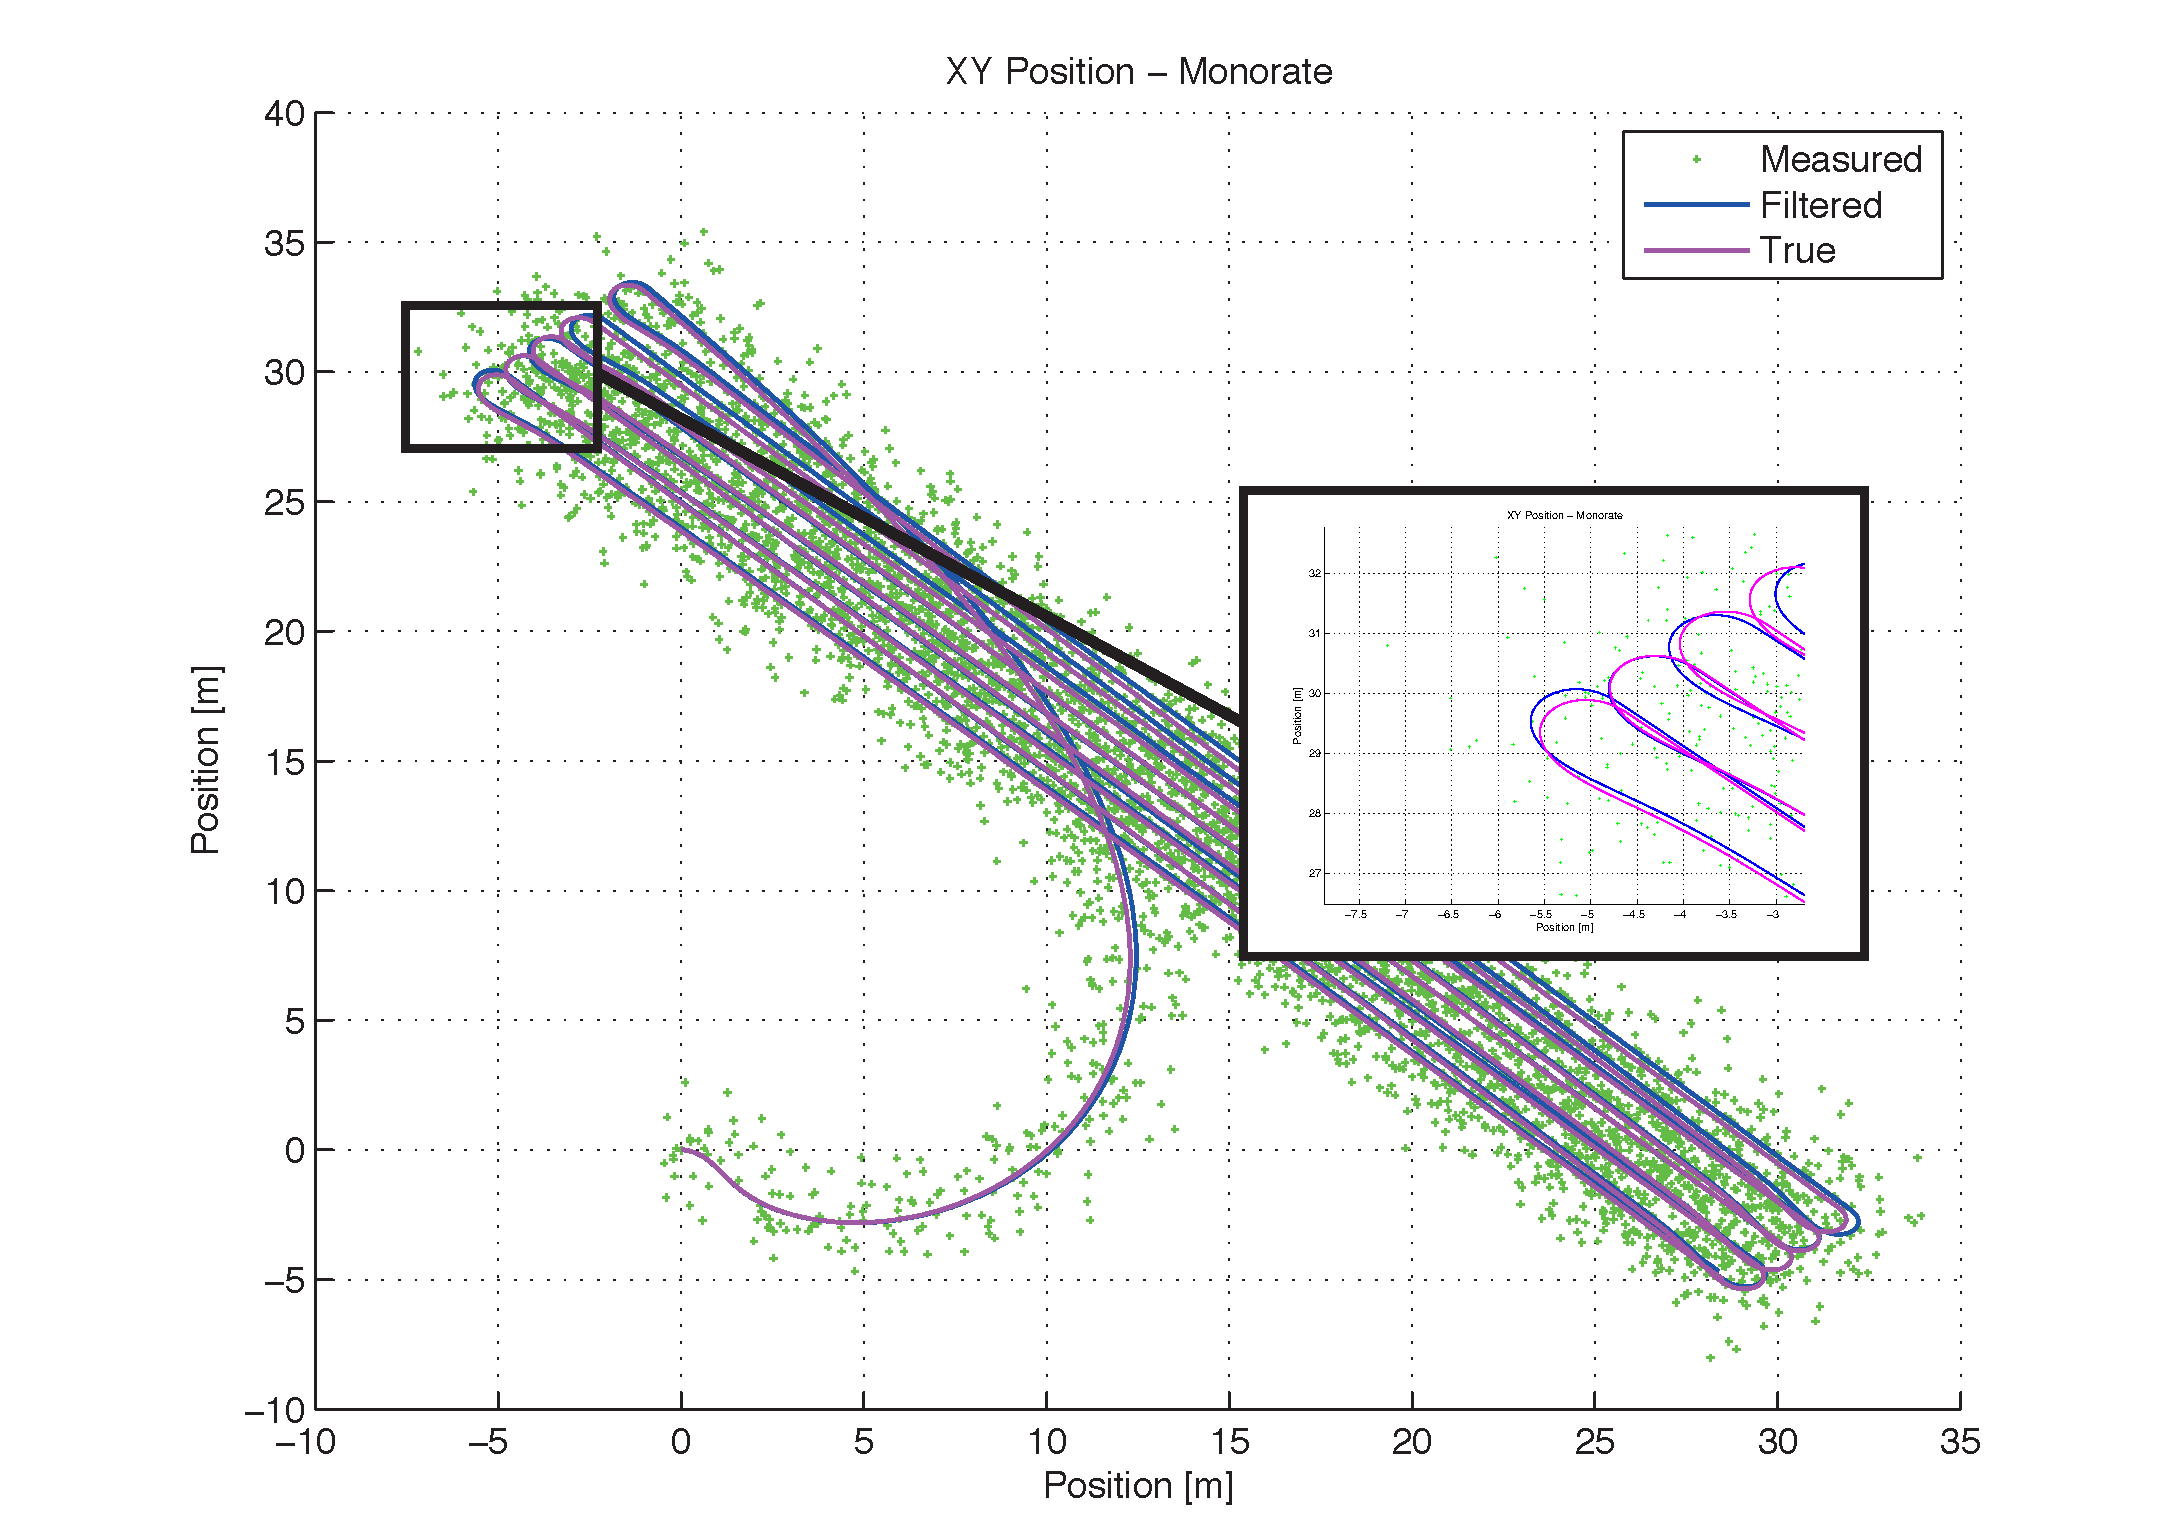
\includegraphics[width=8.2cm]{img/xymono}
					\label{fig:monoratekalman}
				\end{center}
			\end{figure}
		\end{frame}

%###########################

		\begin{frame}{Kalman filter}{Multirate \& input holding}
			\begin{itemize}
				\item The realistic case, using different sampling frequencies
				\item It holds the last GPS position when it does not receive an update
			\end{itemize}
			\begin{figure}
				\begin{center}
					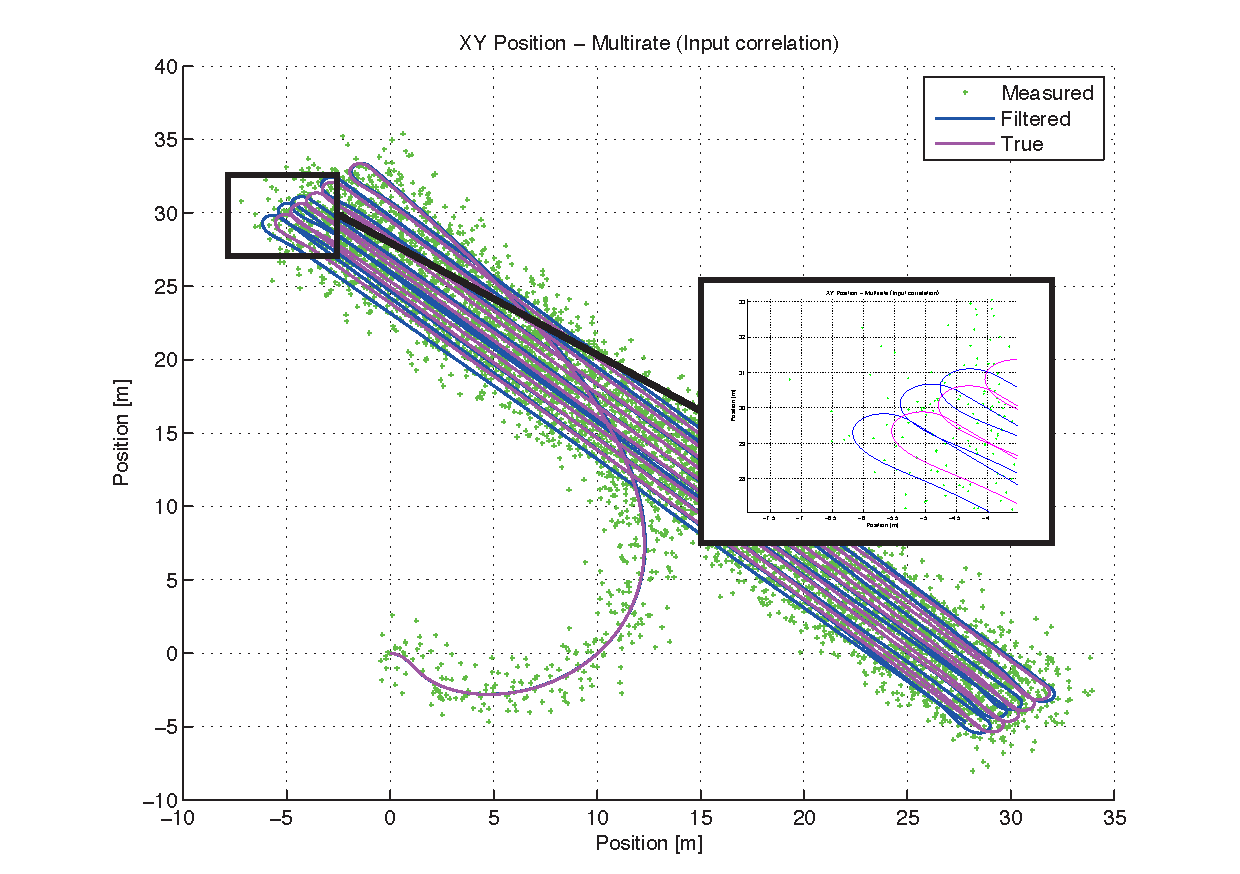
\includegraphics[width=8.2cm]{img/xymnirate}
					\label{fig:multiratekalman1}
				\end{center}
			\end{figure}
		\end{frame}

%###########################

		\begin{frame}{Kalman filter}{Multirate \& input mask}
			The final version: the input mask $ \vec{\Lambda} $ sets the Kalman gain to 0 for invalid inputs.
			\[
		 	\vec{\Lambda} = diag\{\lambda_x,\lambda_{\dot{x}},\lambda_{\ddot{x}},\lambda_{\lambda{y}},\lambda_{\dot{y}},\lambda_{\ddot{y}},\lambda_{\theta},\lambda_{\omega},\lambda_{\alpha} \}
		 	, 
		 	\quad \lambda =  
			 	  \begin{cases}
		 	    1, & \text{valid}\\
		 	    0, & \text{invalid}
			 	  \end{cases}
			\]
			\[
		 	\bar{\vec{K}} = \vec{K} \vec{\Lambda}
		 	\]
			\begin{figure}
				\begin{center}
					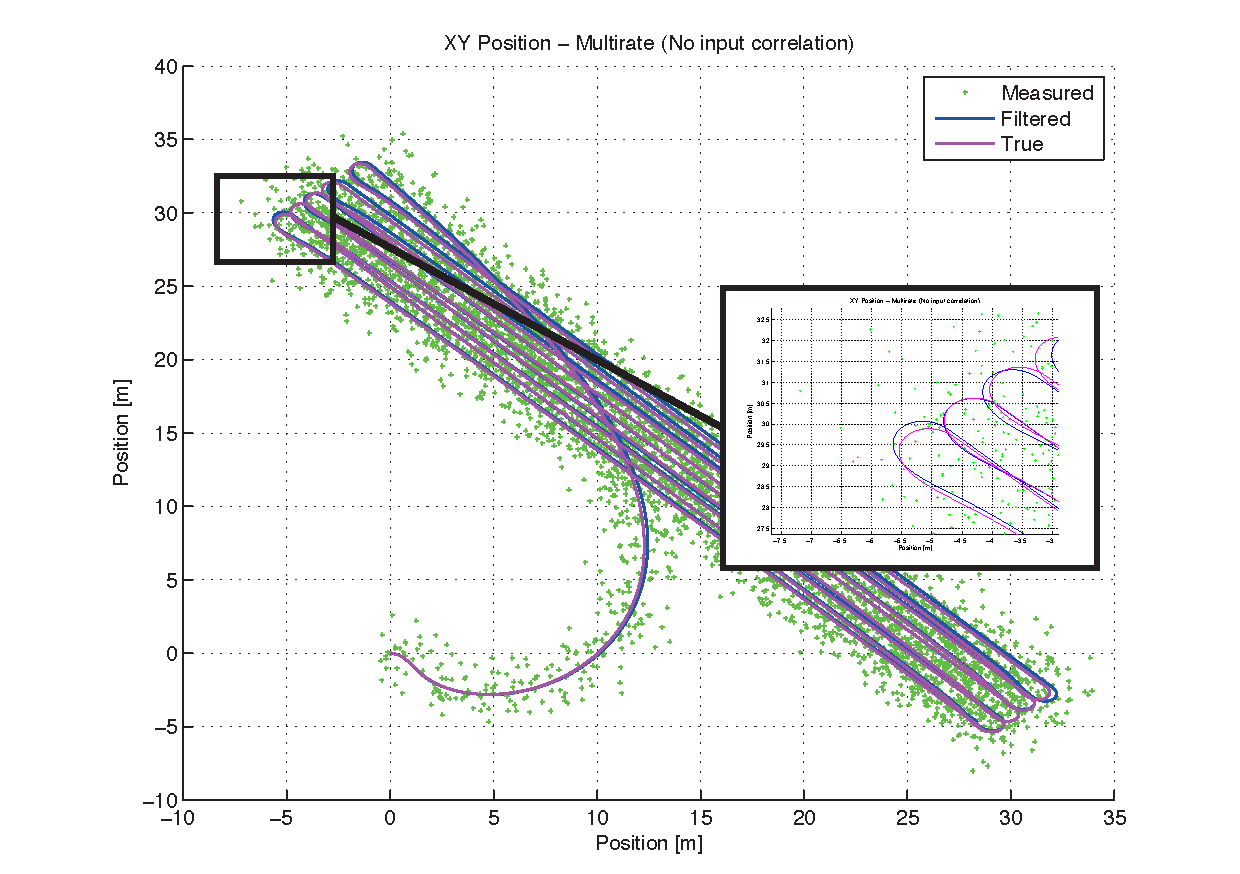
\includegraphics[width=8.2cm]{img/xymultirate}
					\label{fig:multiratekalman2}
				\end{center}
			\end{figure}
		\end{frame}


%###########################

	\subsection{Packet loss}
	% the license
	\begin{frame}{Packet loss}{Considerations}
		\begin{itemize}
			\item<1-> We have a simplex communication link
			\item<2-> It does not guarantee packet arrival or integrity
			\item<3-> It implements a CRC so we can detect errors
			\item<4-> We take advantage of the Kalman filter state estimation
		\end{itemize}
	\end{frame}

%###########################

	\begin{frame}{Packet loss}{Advantages of Kalman filtering}
		\begin{itemize}
			\item Missing GPS samples
			\item Better than simple estimation 
		\end{itemize}
		\begin{figure}
			\begin{center}
				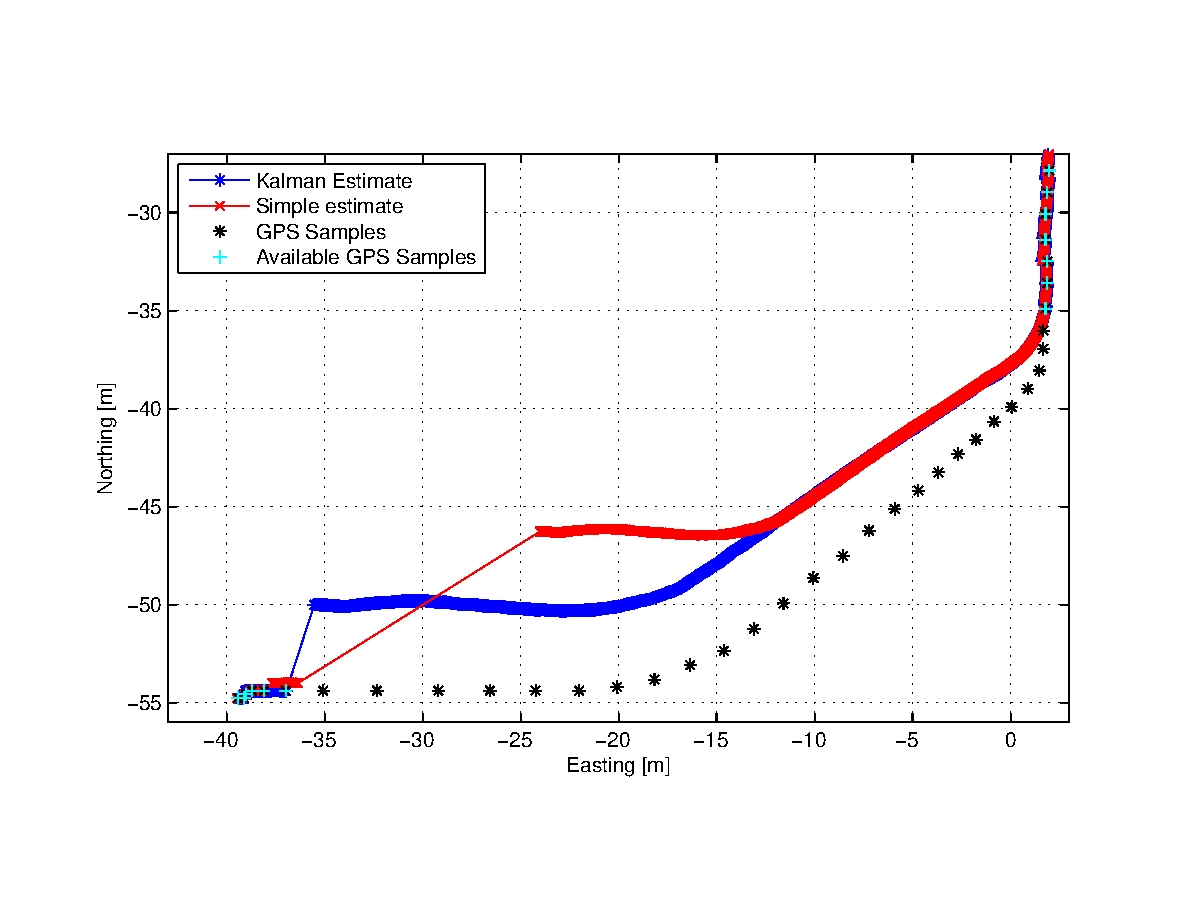
\includegraphics[width=8.2cm]{img/kalmanestimate}
				\label{fig:kalmanestimate}
			\end{center}
		\end{figure}
	\end{frame}
		
%###########################

	\begin{frame}{Packet loss}{Simulation Results}
	  \begin{itemize}
	  	\item Even with and enormously exaggerated packet loss of 100\% for 60 seconds, the Kalman filter still gives a relatively good approximation:
		\begin{figure}
			\begin{center}
				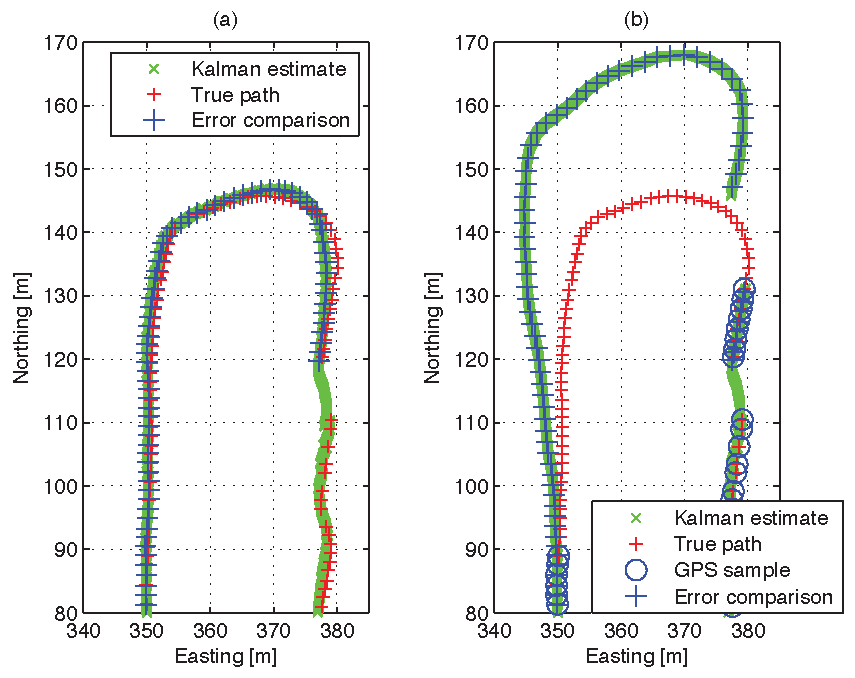
\includegraphics[width=8.2cm]{img/track}
				\label{fig:packetloss}
			\end{center}
		\end{figure}
	  \end{itemize}
	\end{frame}

%###########################

	\begin{frame}{Packet loss}{Simulation Results}
		\begin{itemize}
		  	\item As can be seen, the peak error is around 23 m, which is acceptable
			\begin{figure}
				\begin{center}
					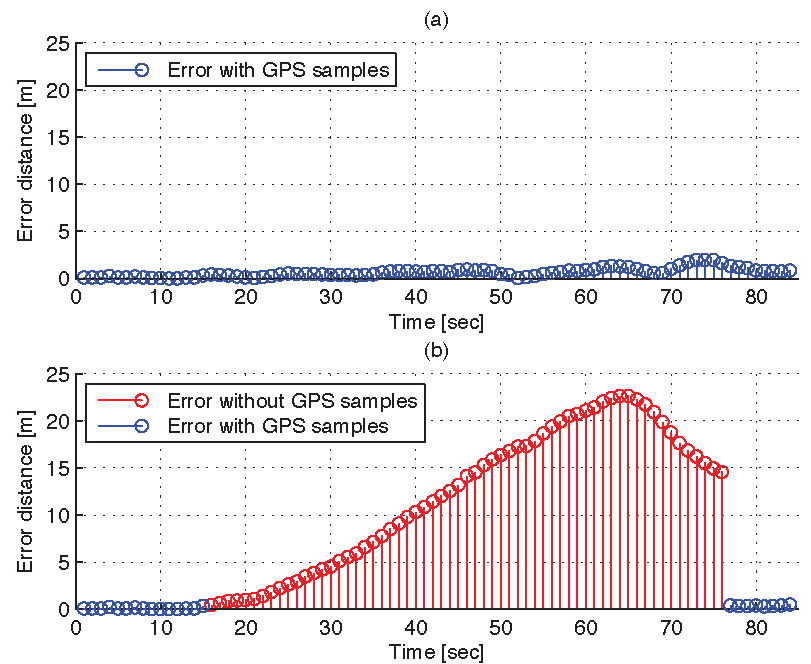
\includegraphics[width=8.2cm]{img/error}
					\label{fig:error}
				\end{center}
			\end{figure}
		\end{itemize}
	\end{frame}

%###########################

	\subsection{Mayden voyage}
	% the license
	\begin{frame}{Mayden voyage}{Purpose and results}
	%  \begin{block}{Ship development}
	  Tested various parts of the ship design and functionality:
	  \begin{itemize}
	  	\item Manual control over wireless link
	  	\item Motor operation and performance
		\item Turning capability and ship stability
		\item Data logging
	  	\end{itemize}
	  	We also added weights to correct its pitch.
	%  \end{block}
		\begin{figure}
			\begin{center}
				\includegraphics[width=9.5cm, trim=0 0 0 50]{img/aauship8}
				\label{fig:aauship}
			\end{center}
		\end{figure}
	\end{frame}

%###########################

	\subsection{Control test}
	\begin{frame}{Testing the control algorithms}{Purpose and results}
		Tested the HLI's waypoint and subwaypoint planning algorithms:
		\begin{itemize}
		\item The ship sailing in Klingenberg lake
		\end{itemize}
		\begin{figure}
			\begin{center}
				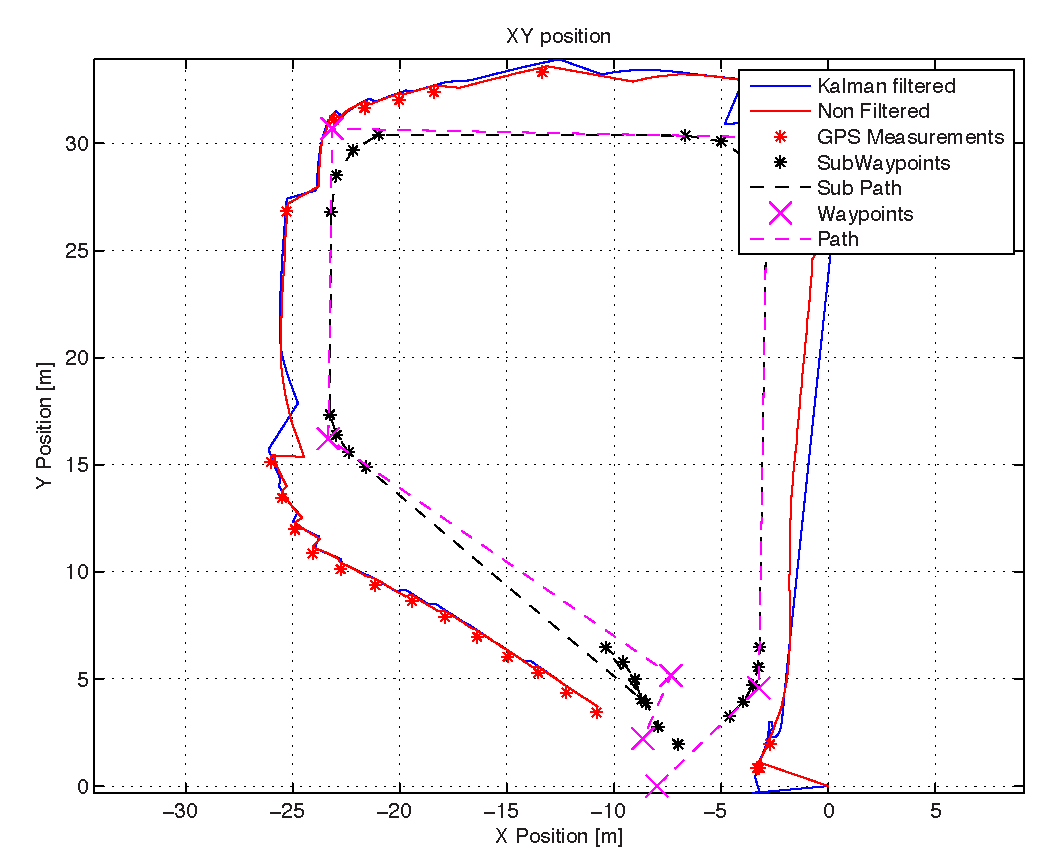
\includegraphics[width=8.2cm]{img/position}
				\label{fig:controltest1}
			\end{center}
		\end{figure}
	\end{frame}

%###########################

	\begin{frame}{Testing the control algorithms}{Results}
		\begin{itemize}
		\item Plot of the ship states during the voyage
		\end{itemize}
		\begin{figure}
			\begin{center}
				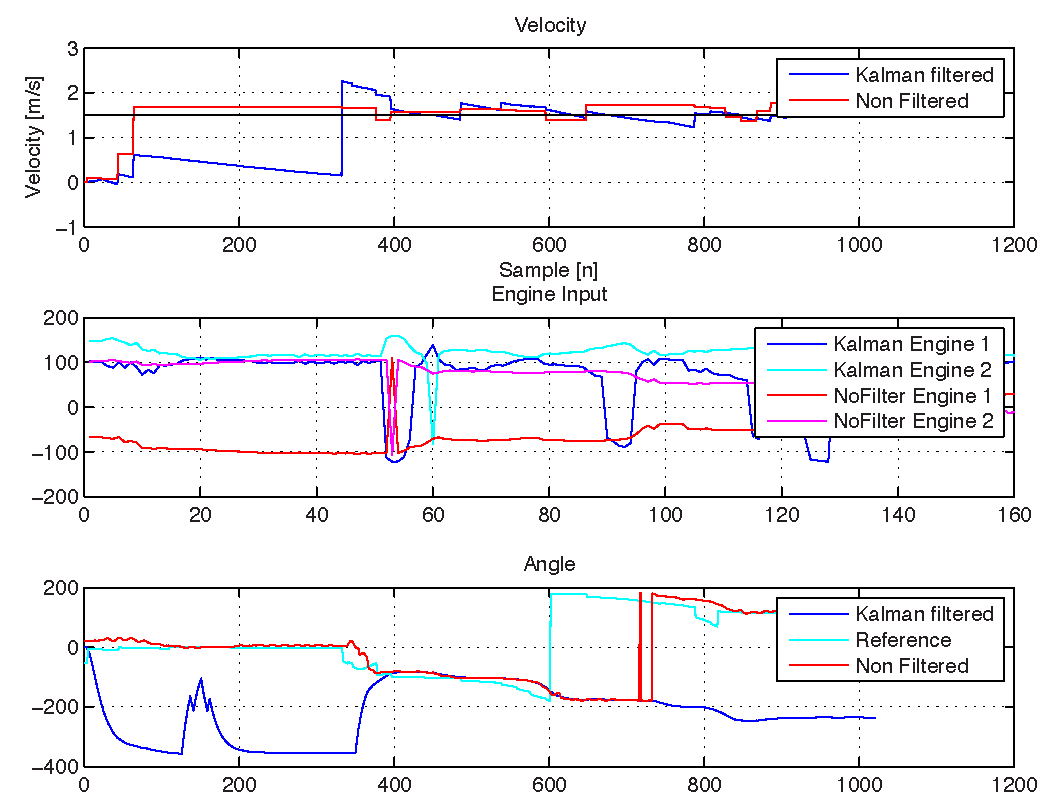
\includegraphics[width=8.2cm]{img/states}
				\label{fig:controltest3}
			\end{center}
		\end{figure}
	\end{frame}

%###########################

	\section{Demonstration}
	\begin{frame}{Demonstration}{}
		Long exposure photo:
		\begin{figure}
			\begin{center}
				\includegraphics[width=9.6cm]{img/aauship}
				\label{fig:aauship1}
			\end{center}
		\end{figure}
		Next: video of the ship sailing autonomously in lake Klingenberg
	\end{frame}